% Graphic for TeX using PGF
% Title: /home/satenske/Diagram2.dia
% Creator: Dia v0.97.1
% CreationDate: Thu Sep 15 10:36:57 2011
% For: satenske
% \usepackage{tikz}
% The following commands are not supported in PSTricks at present
% We define them conditionally, so when they are implemented,
% this pgf file will use them.
\ifx\du\undefined
  \newlength{\du}
\fi
\setlength{\du}{15\unitlength}
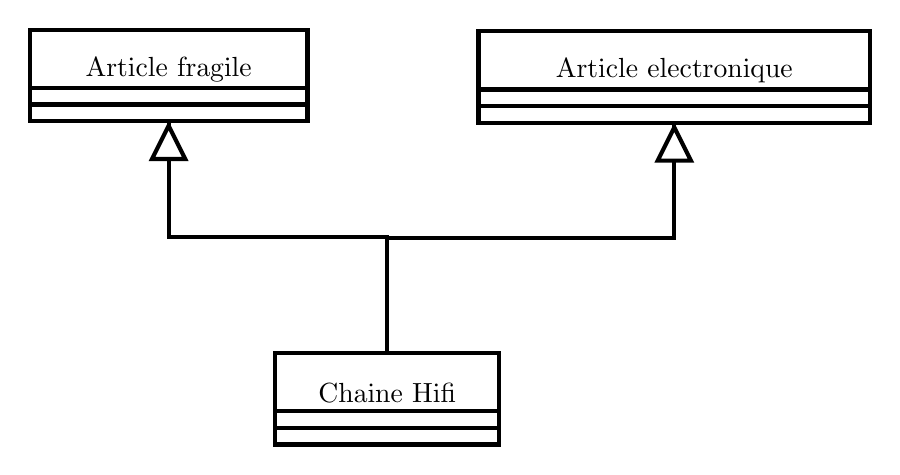
\begin{tikzpicture}
\pgftransformxscale{1.000000}
\pgftransformyscale{-1.000000}
\definecolor{dialinecolor}{rgb}{0.000000, 0.000000, 0.000000}
\pgfsetstrokecolor{dialinecolor}
\definecolor{dialinecolor}{rgb}{1.000000, 1.000000, 1.000000}
\pgfsetfillcolor{dialinecolor}
\pgfsetlinewidth{0.100000\du}
\pgfsetdash{}{0pt}
\definecolor{dialinecolor}{rgb}{1.000000, 1.000000, 1.000000}
\pgfsetfillcolor{dialinecolor}
\fill (4.050000\du,3.550000\du)--(4.050000\du,4.950000\du)--(10.740000\du,4.950000\du)--(10.740000\du,3.550000\du)--cycle;
\definecolor{dialinecolor}{rgb}{0.000000, 0.000000, 0.000000}
\pgfsetstrokecolor{dialinecolor}
\draw (4.050000\du,3.550000\du)--(4.050000\du,4.950000\du)--(10.740000\du,4.950000\du)--(10.740000\du,3.550000\du)--cycle;
% setfont left to latex
\definecolor{dialinecolor}{rgb}{0.000000, 0.000000, 0.000000}
\pgfsetstrokecolor{dialinecolor}
\node at (7.395000\du,4.500000\du){Article fragile};
\definecolor{dialinecolor}{rgb}{1.000000, 1.000000, 1.000000}
\pgfsetfillcolor{dialinecolor}
\fill (4.050000\du,4.950000\du)--(4.050000\du,5.350000\du)--(10.740000\du,5.350000\du)--(10.740000\du,4.950000\du)--cycle;
\definecolor{dialinecolor}{rgb}{0.000000, 0.000000, 0.000000}
\pgfsetstrokecolor{dialinecolor}
\draw (4.050000\du,4.950000\du)--(4.050000\du,5.350000\du)--(10.740000\du,5.350000\du)--(10.740000\du,4.950000\du)--cycle;
\definecolor{dialinecolor}{rgb}{1.000000, 1.000000, 1.000000}
\pgfsetfillcolor{dialinecolor}
\fill (4.050000\du,5.350000\du)--(4.050000\du,5.750000\du)--(10.740000\du,5.750000\du)--(10.740000\du,5.350000\du)--cycle;
\definecolor{dialinecolor}{rgb}{0.000000, 0.000000, 0.000000}
\pgfsetstrokecolor{dialinecolor}
\draw (4.050000\du,5.350000\du)--(4.050000\du,5.750000\du)--(10.740000\du,5.750000\du)--(10.740000\du,5.350000\du)--cycle;
\pgfsetlinewidth{0.100000\du}
\pgfsetdash{}{0pt}
\definecolor{dialinecolor}{rgb}{1.000000, 1.000000, 1.000000}
\pgfsetfillcolor{dialinecolor}
\fill (14.860000\du,3.590000\du)--(14.860000\du,4.990000\du)--(24.295000\du,4.990000\du)--(24.295000\du,3.590000\du)--cycle;
\definecolor{dialinecolor}{rgb}{0.000000, 0.000000, 0.000000}
\pgfsetstrokecolor{dialinecolor}
\draw (14.860000\du,3.590000\du)--(14.860000\du,4.990000\du)--(24.295000\du,4.990000\du)--(24.295000\du,3.590000\du)--cycle;
% setfont left to latex
\definecolor{dialinecolor}{rgb}{0.000000, 0.000000, 0.000000}
\pgfsetstrokecolor{dialinecolor}
\node at (19.577500\du,4.540000\du){Article electronique};
\definecolor{dialinecolor}{rgb}{1.000000, 1.000000, 1.000000}
\pgfsetfillcolor{dialinecolor}
\fill (14.860000\du,4.990000\du)--(14.860000\du,5.390000\du)--(24.295000\du,5.390000\du)--(24.295000\du,4.990000\du)--cycle;
\definecolor{dialinecolor}{rgb}{0.000000, 0.000000, 0.000000}
\pgfsetstrokecolor{dialinecolor}
\draw (14.860000\du,4.990000\du)--(14.860000\du,5.390000\du)--(24.295000\du,5.390000\du)--(24.295000\du,4.990000\du)--cycle;
\definecolor{dialinecolor}{rgb}{1.000000, 1.000000, 1.000000}
\pgfsetfillcolor{dialinecolor}
\fill (14.860000\du,5.390000\du)--(14.860000\du,5.790000\du)--(24.295000\du,5.790000\du)--(24.295000\du,5.390000\du)--cycle;
\definecolor{dialinecolor}{rgb}{0.000000, 0.000000, 0.000000}
\pgfsetstrokecolor{dialinecolor}
\draw (14.860000\du,5.390000\du)--(14.860000\du,5.790000\du)--(24.295000\du,5.790000\du)--(24.295000\du,5.390000\du)--cycle;
\pgfsetlinewidth{0.100000\du}
\pgfsetdash{}{0pt}
\definecolor{dialinecolor}{rgb}{1.000000, 1.000000, 1.000000}
\pgfsetfillcolor{dialinecolor}
\fill (9.960000\du,11.340000\du)--(9.960000\du,12.740000\du)--(15.360000\du,12.740000\du)--(15.360000\du,11.340000\du)--cycle;
\definecolor{dialinecolor}{rgb}{0.000000, 0.000000, 0.000000}
\pgfsetstrokecolor{dialinecolor}
\draw (9.960000\du,11.340000\du)--(9.960000\du,12.740000\du)--(15.360000\du,12.740000\du)--(15.360000\du,11.340000\du)--cycle;
% setfont left to latex
\definecolor{dialinecolor}{rgb}{0.000000, 0.000000, 0.000000}
\pgfsetstrokecolor{dialinecolor}
\node at (12.660000\du,12.290000\du){Chaine Hifi};
\definecolor{dialinecolor}{rgb}{1.000000, 1.000000, 1.000000}
\pgfsetfillcolor{dialinecolor}
\fill (9.960000\du,12.740000\du)--(9.960000\du,13.140000\du)--(15.360000\du,13.140000\du)--(15.360000\du,12.740000\du)--cycle;
\definecolor{dialinecolor}{rgb}{0.000000, 0.000000, 0.000000}
\pgfsetstrokecolor{dialinecolor}
\draw (9.960000\du,12.740000\du)--(9.960000\du,13.140000\du)--(15.360000\du,13.140000\du)--(15.360000\du,12.740000\du)--cycle;
\definecolor{dialinecolor}{rgb}{1.000000, 1.000000, 1.000000}
\pgfsetfillcolor{dialinecolor}
\fill (9.960000\du,13.140000\du)--(9.960000\du,13.540000\du)--(15.360000\du,13.540000\du)--(15.360000\du,13.140000\du)--cycle;
\definecolor{dialinecolor}{rgb}{0.000000, 0.000000, 0.000000}
\pgfsetstrokecolor{dialinecolor}
\draw (9.960000\du,13.140000\du)--(9.960000\du,13.540000\du)--(15.360000\du,13.540000\du)--(15.360000\du,13.140000\du)--cycle;
\pgfsetlinewidth{0.100000\du}
\pgfsetdash{}{0pt}
\pgfsetmiterjoin
\pgfsetbuttcap
{
\definecolor{dialinecolor}{rgb}{0.000000, 0.000000, 0.000000}
\pgfsetfillcolor{dialinecolor}
% was here!!!
\definecolor{dialinecolor}{rgb}{0.000000, 0.000000, 0.000000}
\pgfsetstrokecolor{dialinecolor}
\draw (7.395000\du,5.750000\du)--(7.395000\du,8.545000\du)--(12.660000\du,8.545000\du)--(12.660000\du,11.340000\du);
}
\definecolor{dialinecolor}{rgb}{0.000000, 0.000000, 0.000000}
\pgfsetstrokecolor{dialinecolor}
\draw (7.395000\du,6.661803\du)--(7.395000\du,8.545000\du)--(12.660000\du,8.545000\du)--(12.660000\du,11.340000\du);
\pgfsetmiterjoin
\definecolor{dialinecolor}{rgb}{1.000000, 1.000000, 1.000000}
\pgfsetfillcolor{dialinecolor}
\fill (7.795000\du,6.661803\du)--(7.395000\du,5.861803\du)--(6.995000\du,6.661803\du)--cycle;
\pgfsetlinewidth{0.100000\du}
\pgfsetdash{}{0pt}
\pgfsetmiterjoin
\definecolor{dialinecolor}{rgb}{0.000000, 0.000000, 0.000000}
\pgfsetstrokecolor{dialinecolor}
\draw (7.795000\du,6.661803\du)--(7.395000\du,5.861803\du)--(6.995000\du,6.661803\du)--cycle;
% setfont left to latex
\pgfsetlinewidth{0.100000\du}
\pgfsetdash{}{0pt}
\pgfsetmiterjoin
\pgfsetbuttcap
{
\definecolor{dialinecolor}{rgb}{0.000000, 0.000000, 0.000000}
\pgfsetfillcolor{dialinecolor}
% was here!!!
\definecolor{dialinecolor}{rgb}{0.000000, 0.000000, 0.000000}
\pgfsetstrokecolor{dialinecolor}
\draw (19.577500\du,5.790000\du)--(19.577500\du,8.565000\du)--(12.660000\du,8.565000\du)--(12.660000\du,11.340000\du);
}
\definecolor{dialinecolor}{rgb}{0.000000, 0.000000, 0.000000}
\pgfsetstrokecolor{dialinecolor}
\draw (19.577500\du,6.701803\du)--(19.577500\du,8.565000\du)--(12.660000\du,8.565000\du)--(12.660000\du,11.340000\du);
\pgfsetmiterjoin
\definecolor{dialinecolor}{rgb}{1.000000, 1.000000, 1.000000}
\pgfsetfillcolor{dialinecolor}
\fill (19.977500\du,6.701803\du)--(19.577500\du,5.901803\du)--(19.177500\du,6.701803\du)--cycle;
\pgfsetlinewidth{0.100000\du}
\pgfsetdash{}{0pt}
\pgfsetmiterjoin
\definecolor{dialinecolor}{rgb}{0.000000, 0.000000, 0.000000}
\pgfsetstrokecolor{dialinecolor}
\draw (19.977500\du,6.701803\du)--(19.577500\du,5.901803\du)--(19.177500\du,6.701803\du)--cycle;
% setfont left to latex
\end{tikzpicture}
